\chapter{Área de estudo}
\label{capArea}
\hspace{2.0cm} O complexo sedimentar das bacias do Iguatu compreende um conjunto de quatro sub-bacias localizadas geograficamente na porção sudeste do Estado do Ceará, entre as coordenadas geográficas de Latitude $6^{\circ}$ $06' 36''$ S e $6^{\circ}$ $28' 06''$ S e de longitude $39 ^{\circ}$ $27' 06''$ W e $38^{\circ}$ $39' 18''$ W Figura \ref{fig:localizacao_igatu}.
 O conjunto de sub-bacias constitui uma área de cerca de 1318 $Km^{2}$, são denominadas Iguatu, Malhada Vermelha, Lima Campos e Icó, todas com eixo principal na direção NE-SW. A sub-bacia do Iguatu é a maior entre as quatro, está situada na porção ocidental em relação às demais, ocupa uma área de aproximadamente $820$ $km^{2}$ e tem um formato aproximadamente elíptico, apresentando cerca de $57$ $Km$ de comprimento no eixo maior e $23$ $Km$ no eixo menor, o que corresponde cerca de $70\%$ da área total do complexo sedimentar. 

A gênese e evolução da bacia do Iguatu, assim como das outras bacias interiores do Nordeste estão relacionadas à fase inicial de abertura do Proto-oceano Atlântico (Evento Sul Atlantiano – 160-115 Ma) durante o final do Jurássico e início do Cretáceo \citep{naoki2007}.

O embasamento cristalino é formado por diferentes domínios estruturais pertencentes à Província Borborema Figura \ref{fig:borboreema}, esses domínios encontram-se intensamente deformados e dominados por zonas de cisalhamento de idades neoproterozóicas. A reativação Eocretácica destas zonas durante o processo de rifteamento intracontinental mesozóico, associado à abertura e formação do Atlântico Sul, condicionou a estruturação interna das bacias intracratônicas \citep{castro99}.
 
 
 
\begin{figure}[h]
\centering
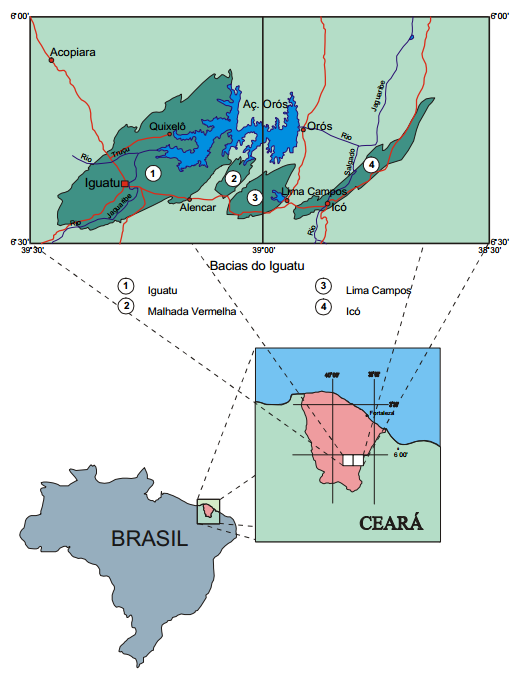
\includegraphics[width=1.0\linewidth]{Figs/baciasdo_iguatu}
\caption{Mapa de localização das sub-bacias Iguatu, Malhada Vermelha, Lima Campos e Icó que compreendem a bacia de Iguatu, porção sudeste do estado do Ceará, \citep{Ribeiro_2000}.}
\label{fig:localizacao_igatu}
\end{figure}



\begin{figure}
\centering
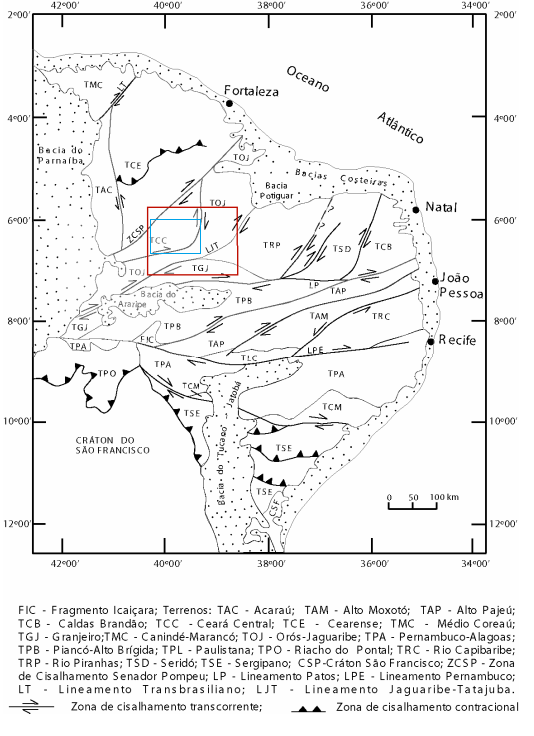
\includegraphics[width=1.0\linewidth]{Figs/borboreema}
\caption{Principais terrenos tectono-estratigráficos da Província Borborema, com a área de estudo em destaque. \citep{naoki2007} apud. (JARDIM DE SÁ, 1994) e SANTOS et al. 1998)}
\label{fig:borboreema}
\end{figure}


%\begin{figure}
%\centering
%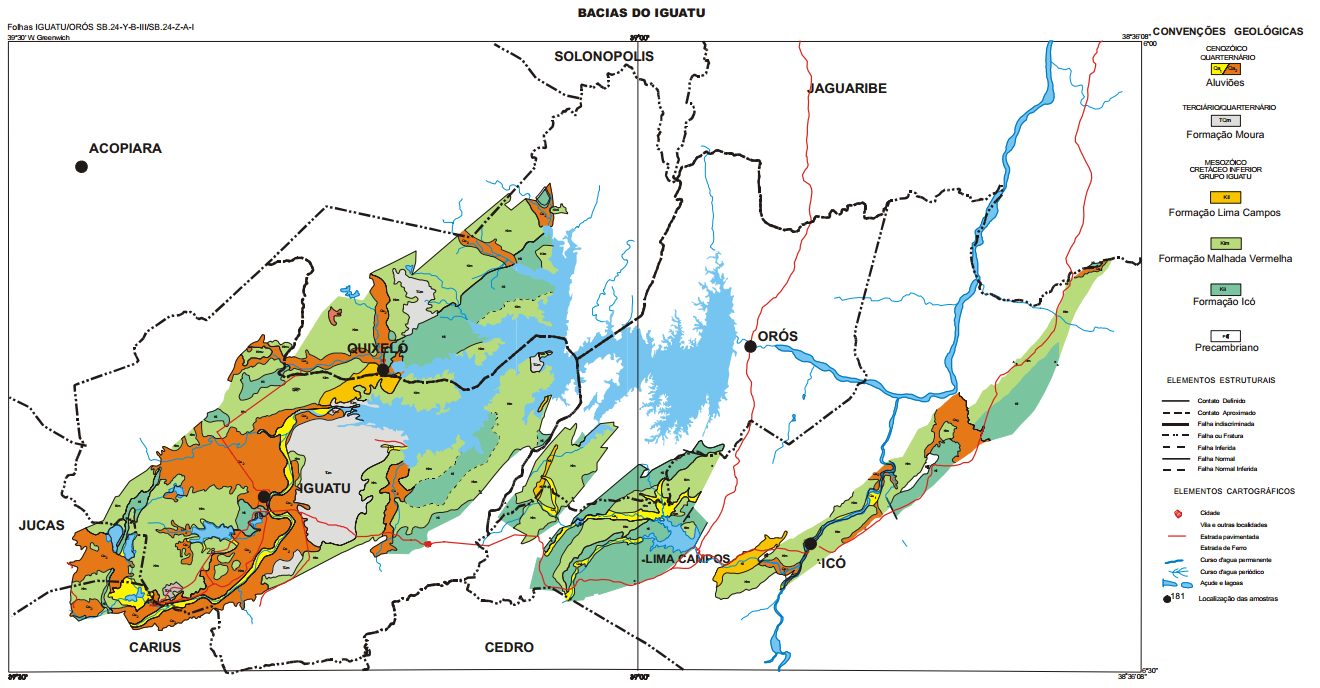
\includegraphics[width=1.4\linewidth, %height=0.5\textheight,angle=90]{Figs/geologia_iguatu_cprm}
%\caption{ Mapa geológico das bacias do Iguatu \citep{cprm}.}
%\label{fig:geologia_iguatu_cprm}
%\end{figure}







%As bacias do Iguatu representam parte das coberturas sedimentares mesozóicas inseridas na Região de Dobramentos Nordeste ou Província Borborema, tal como as bacias do Araripe e Rio do Peixe, além de outras menores (Pontes Filho, 1996). A Província Borborema tem cerca de 400.000km2 cobrindo a região nordeste oriental do Brasil, desde o norte da Bahia até o noroeste do Ceará. É limitada regionalmente pelos crátons de São Francisco, ao sul e de São Luis, à noroeste. Estruturalmente, a Província Borborema caracteriza-se por um complexo conjunto de lineamentos de direções variadas, que a cortam dividindo-a em zonas de geofraturas de direção predominantemente NE-SW. Não existe consenso a respeito da estratigrafia das bacias do Iguatu. Mabesoone e Campanha (1974) optaram pela denominação Grupo Iguatu, subdivido em três formações: Quixoá (inferior), Malhada Vermelha (intermediária) e Lima Campos (superior). Esses autores sugeriram uma idade entre o Jurássico Superior e o Cretáceo inferior para o Grupo Iguatu. Outros autores (Campos et al., 1979; Gomes et al., 1981) agruparam as várias bacias interiores como sendo pertencentes ao Grupo Rio Peixe, interpretando-as como representantes de uma área de sedimentação contínua em tempos passados com extraordinária identidade estratigráfica e paleogeográfica, além de características lito-faciológicas e evolução tectônica semelhante. O trabalho mais recente (Srivastava, 1990) subdivide a bacia do Iguatu em três unidades estratigráficas informais (I, II e III), sendo a unidade I (basal) constituída de arenitos médios a muitos grossos, com níveis conglomeráticos a conglomerados, apresentando espessura estimada da ordem de 200 m. A unidade II é a de maior predominância na bacia, possuindo espessura inferida da ordem de 1000m. Sua constituição inclui arenitos finos, intercalados por siltitos e folhelhos, arenitos grossos a conglomeráticos associados e interdigitados, com pequena presença de siltitos e folhelhos; arenitos bimodais e finos; folhelhos e calcários, intercalados. A unidade III apresenta espessura mínima de 150 m, sendo constituída por arenitos grossos e níveis síltico-argilosos. Sobrepondo a estas unidades da Bacia do Iguatu ocorrem sedimentos terciários e quaternários da Formação Moura.








%\begin{equation}
%	\frac{\partial Y}{\partial t}
%\end{equation}

%\begin{itemize}
%	\item Nelson
%	\item Vitor
%\end{itemize}
%\begin{table}[h]
%\caption[Exemplos de tabela (texto do índice)]{Exemplos de tabela mostrando os comandos para
 % cita{\c c}\~oes utilizando o comando padr\~ao \texttt{\textbackslash citep} do \LaTeX\ e
  %o comando \texttt{\textbackslash citet},
  %fornecido pelo pacote \texttt{natbib}.}
%\label{tab:citation}
%\centering
%{\footnotesize
%\begin{tabular}{|c|c|c|}
 % \hline
  %Tipo da Publica{\c c}\~ao & \verb|\citep| & \verb|\citet|\\
  %\hline
  %Livro & \citep{book-example} & \citet{book-example}\\
  %Artigo & \citep{article-example} & \citet{article-example}\\
 % Relat\'orio & \citep{techreport-example} & \citet{techreport-example}\\
  %Relat\'orio & \citep{techreport-exampleIn} & \citet{techreport-exampleIn}\\
  %Anais de Congresso & \citep{inproceedings-example} &
   % \citet{inproceedings-example}\\
  %S\'eries & \citep{incollection-example} & \citet{incollection-example}\\
 % Em Livro & \citep{inbook-example} & \citet{inbook-example}\\
  %Disserta{\c c}\~ao de mestrado & \citep{mastersthesis-example} &
   % \citet{mastersthesis-example}\\
  %Tese de doutorado & \citep{phdthesis-example} & \citet{phdthesis-example}\\
  %\hline
%\end{tabular}}
%\end{table}


